\section{Published efficient SR models on small ear images}
\label{sec:analysis}

\subsection{The advantage over interpolation disappears under compression}
Table~\ref{tab:published} reports the \NPub{} fidelity-oriented models at the main cell of AMI. On clean inputs they behave as their design intends: every model exceeds bicubic interpolation, by \AmiCleanGainMin{} to \AmiCleanGainMax{}~dB. The picture changes with compression (Figure~\ref{fig:sweep}). At JPEG quality 93 the gain shrinks to \AmiQHighGainMin{} to \AmiQHighGainMax{}~dB. At quality 85 every model is below bicubic, by \AmiQMidGapMin{} to \AmiQMidGapMax{}~dB, and at quality 75 by \AmiQLowGapMin{} to \AmiQLowGapMax{}~dB. SPAN, for example, drops from \SpanCleanPsnr{} to \SpanQLowPsnr{}~dB, while bicubic interpolation drops only from \BicCleanPsnr{} to \BicQLowPsnr{}~dB. We attribute this to a network trained to sharpen clean bicubic inputs also sharpening the blocking artefacts that interpolation smooths \todo{support with the error-spectrum figure}.

\begin{table}[t]
\centering
\caption{Models with public weights on AMI at $\times4$ with 36-pixel inputs (\NAmiAllImg{} images). PSNR-Y in dB; values above bicubic interpolation are in bold. Latency is the median over single $48\times68$ inputs on an RTX~3080 in 32-bit precision. The lower block lists GAN-trained models.}
\label{tab:published}
\resizebox{\linewidth}{!}{%
\begin{tabular}{@{}lrrcccrr@{}}
\toprule
 & Params & Latency & \multicolumn{3}{c}{PSNR-Y, by input} & \multicolumn{2}{c}{LPIPS, by input} \\
\cmidrule(lr){4-6}\cmidrule(l){7-8}
Model & (K) & (ms) & Clean & JPEG 93 & JPEG 75 & Clean & JPEG 75 \\
\midrule
\tabinput{generated/tab_published}
\bottomrule
\end{tabular}}
\end{table}

\begin{figure}[t]
\centering
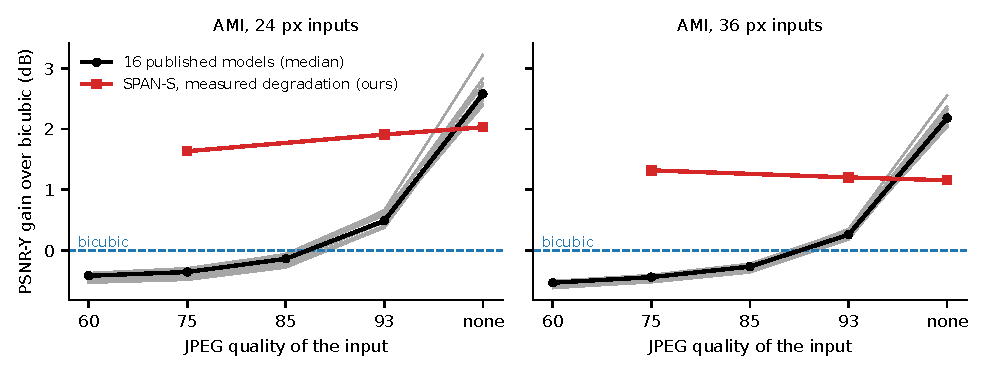
\includegraphics[width=\linewidth]{figures/fig_jpeg_sweep.pdf}
\caption{PSNR gain over bicubic interpolation as a function of the JPEG quality of the input, on AMI. Grey: each of the \NPub{} published fidelity-oriented models (\NAmiAllImg{} images); black: their median. Red: SPAN fine-tuned with the measured degradation (Section~\ref{sec:method}; each model on the test subjects of its fold).}
\label{fig:sweep}
\end{figure}

\subsection{The effect is not specific to one dataset or one input size}
Table~\ref{tab:generality} repeats the comparison at the three input sizes of AMI and on the two in-the-wild datasets. At quality 75, all \NPub{} models are significantly below bicubic at every input size of AMI and on AWEx at both sizes. On EarVN1.0 the mean gain is negative for \EarvnQLowBelow{} of the \NPub{} models and significantly so for \EarvnQLowSig{}; the remaining models are statistically tied with interpolation. At quality 93 no model is below bicubic on any dataset. Under the measured degradation, which mixes the two levels, the published models are within \WildEstGainMin{} to \WildEstGainMax{}~dB of bicubic on the in-the-wild sets, compared with a gain of \WildCleanGainMin{} to \WildCleanGainMax{}~dB on clean inputs. We therefore state the finding as follows: \emph{on small ear images, bicubic-trained SR models lose their fidelity advantage over interpolation under realistic compression, and fall below it from a JPEG quality of about 85 downwards}. The deficit does not grow as the input shrinks (SPAN: \SpanQLowGapS{}, \SpanQLowGapM{} and \SpanQLowGapL{}~dB at 24, 36 and 48 pixels); it is a property of the compression, present at every size we test.

\begin{table}[t]
\centering
\caption{Median PSNR gain over bicubic interpolation of the \NPub{} published fidelity-oriented models (dB), by dataset, input size and input degradation. In parentheses: number of models whose mean gain is negative / number whose 95\% confidence interval lies entirely below zero. ``--'': not evaluated.}
\label{tab:generality}
\resizebox{\linewidth}{!}{%
\begin{tabular}{@{}lrrccccc@{}}
\toprule
Dataset & Input (px) & Images & Clean & JPEG 93 & JPEG 85 & JPEG 75 & Measured \\
\midrule
\tabinput{generated/tab_generality}
\bottomrule
\end{tabular}}
\end{table}

\subsection{Ears, small inputs, or compression? A control on natural images}
\label{sec:natural}
Three things distinguish our benchmark from the protocol under which these models were trained: the content (ears), the input size (a few dozen pixels) and the compression. To separate them we evaluate the same \NPub{} models on natural images: the \NatN{} validation images of DIV2K~\cite{agustsson2017div2k}, each downsized to inputs of 24 to \NatLargePx{} pixels and degraded with the same JPEG levels (Table~\ref{tab:natural}). No model is trained or added for this control. The result separates the three factors. \emph{Input size does not move the crossover.} At JPEG quality 75 every model remains above bicubic interpolation on natural images at every input size, with a median gain of \NatSQLowMed{}~dB at 36-pixel inputs and \NatLQLowMed{}~dB at \NatLargePx{}-pixel inputs; at quality 60 every model is below it at every size (\NatSQVLowMed{} and \NatLQVLowMed{}~dB). \emph{Content does.} For natural images the crossover lies between quality 75 and 60; for ear images it lies between 93 and 85. \emph{The collapse of architectural differences is general.} On natural images the \NPub{} models span \NatSpreadCleanS{}~dB on clean 36-pixel inputs and \NatSpreadQLowS{}~dB at quality 75, as they do on ears.

\paragraph{One quantity accounts for both observations} Let $E_i$ be the mean squared error of bicubic interpolation of the clean input, and $E_c$ the additional error of bicubic interpolation when the input is compressed. Figure~\ref{fig:ratio} plots the median gain of the \NPub{} models against the ratio $E_c/E_i$ for all \RatioCells{} combinations of dataset, input size and JPEG quality in the \RatioSets{} datasets (inputs of \RatioPxMin{} to \RatioPxMax{} pixels, quality 60 to 93). In every combination with $E_c/E_i\le\RatioMaxAbove$ all \NPub{} models are above bicubic interpolation; in every combination with $E_c/E_i\ge\RatioMinBelow$ all of them are below it, except on EarVN1.0 at quality 75, where \EarvnQLowBelow{} are. The rank correlation between the ratio and the gain is \RatioSpearman{}. The rationale is simple: an SR network reduces the interpolation error and amplifies the compression error, so it can win only while the second is small relative to the first. Ear images are smooth. Bicubic interpolation of a clean 36-pixel input reaches \BicCleanPsnr{}~dB on AMI against \NatSBicClean{}~dB on DIV2K, so $E_i$ is small and a given JPEG quality contributes a far larger share of the error: at quality 75 the ratio is \RatioAmiQLow{} for AMI and \RatioDivQLow{} for DIV2K, and AMI at quality 93 has the same ratio as DIV2K at quality 60 (\RatioAmiQHigh{} and \RatioDivQVLow{}). What is specific to ear images is therefore not the phenomenon but its location: the compression levels that real small ear images carry lie beyond the threshold, whereas for natural images at the same levels they do not.

The threshold of about \RatioThresh{} is empirical. It is observed for bicubic-trained $\times4$ models and JPEG compression only, and the two combinations closest to it lie on opposite sides at almost the same ratio with gains that differ in size, so the gain is not a function of the ratio alone.

\begin{figure}[t]
\centering
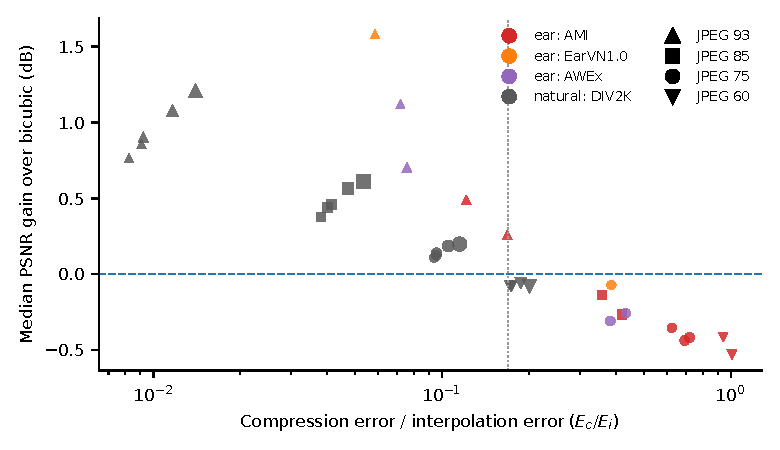
\includegraphics[width=0.8\linewidth]{figures/fig_ratio.pdf}
\caption{Median PSNR gain of the \NPub{} published models over bicubic interpolation against the ratio of compression error to interpolation error, for every dataset, input size (marker size) and JPEG quality. The dotted line marks the empirical threshold.}
\label{fig:ratio}
\end{figure}

\begin{table}[t]
\centering
\caption{Natural images against ear images: median PSNR gain over bicubic interpolation of the \NPub{} published models (dB) by input size and input degradation. In parentheses: number of models with negative mean gain / number significantly below zero.}
\label{tab:natural}
\resizebox{\linewidth}{!}{%
\begin{tabular}{@{}lrrccccc@{}}
\toprule
Images & Input (px) & Images & Clean & JPEG 93 & JPEG 85 & JPEG 75 & JPEG 60 \\
\midrule
\tabinput{generated/tab_natural}
\bottomrule
\end{tabular}}
\end{table}

\subsection{Fidelity and perceptual metrics disagree}
At quality 75, \LpipsQLowBetter{} of the \NPub{} models still have a lower LPIPS than bicubic interpolation (for SPAN, \SpanQLowLpips{} against \BicQLowLpips{}). The outputs look sharper while being further from the ground truth. This matters for how the finding is worded, and for applications: where the enlarged image is evidence, or the input of a recognition system, sharper but less faithful is not obviously an improvement. The perceptual models make the trade explicit. BSRGAN reaches an LPIPS of \BsrganQLowLpips{} at quality 75, the best of all models, at a PSNR \BsrganQLowGap{}~dB below bicubic interpolation and at \LatRatio{} times the latency of SPAN.

\subsection{Architecture is not the bottleneck}
\label{sec:capacity}
On clean inputs the \NPub{} models span \SpreadClean{}~dB and capacity pays: the \ParamsRrdb{}M-parameter RRDB exceeds the \ParamsSpan{}M-parameter SPAN by \RrdbVsSpanCleanL{}, \RrdbVsSpanCleanM{} and \RrdbVsSpanCleanS{}~dB at 48, 36 and 24-pixel inputs, more as the input shrinks. Under JPEG 75 the same models span only \SpreadQLow{}~dB, RRDB is \RrdbVsSpanQLowM{}~dB from SPAN, and the ranking of the models is unrelated to their ranking on clean inputs (Kendall's $\tau=\TauRank$ between the two orderings by mean PSNR). No choice among the published architectures recovers the lost fidelity. Section~\ref{sec:experiments} shows that a change of training degradation on a single architecture does.
